% =====================================================================
% bmr_feynman_linear_algebra.tex
%
% A standalone explainer (not the paper): Bayesian Model Reduction and
% Expansion from a linear-algebra-into-dynamics point of view, in the
% spirit of "build one object and rotate it."
%
% The one object is the INFORMATION (precision) matrix. The two moves are
% BORDERING (add a node / expand) and SCHUR COMPLEMENT (remove a node /
% reduce). The ledger that prices both is the moment generating function.
%
% Compiles standalone:  pdflatex bmr_feynman_linear_algebra
% =====================================================================
\documentclass[11pt]{article}

\usepackage[a4paper,margin=1in]{geometry}
\usepackage[T1]{fontenc}
\usepackage[utf8]{inputenc}
\usepackage{amsmath,amssymb,amsthm,mathtools,bm}
\usepackage{microtype}
\usepackage{xcolor}
\usepackage{tikz}
\usepackage{pgfplots}
\pgfplotsset{compat=1.18}
\usetikzlibrary{arrows.meta,positioning,calc,fit,backgrounds,matrix,
                decorations.pathreplacing,decorations.pathmorphing,shapes.misc}
\usepackage{hyperref}
\hypersetup{colorlinks=true,linkcolor=blue!45!black,citecolor=blue!45!black,urlcolor=blue!45!black}

% ----- palette
\definecolor{infomat}{RGB}{40,70,130}
\definecolor{addcol}{RGB}{60,130,90}
\definecolor{remcol}{RGB}{170,60,60}
\definecolor{amber}{RGB}{200,145,50}
\definecolor{soft}{RGB}{215,225,240}
\definecolor{softg}{RGB}{215,235,225}
\definecolor{softr}{RGB}{240,215,215}
\definecolor{grey}{RGB}{95,95,110}

% ----- notation
\newcommand{\R}{\mathbb{R}}
\newcommand{\E}{\mathbb{E}}
\newcommand{\KL}[2]{D_{\mathrm{KL}}\!\left(#1\,\middle\|\,#2\right)}
\newcommand{\Prec}{\bm{\Pi}}        % precision / information matrix
\newcommand{\Cov}{\bm{\Sigma}}
\newcommand{\hvec}{\bm{h}}          % potential vector = Pi mu
\newcommand{\fvec}{\bm{\varphi}}    % parameters
\newcommand{\Z}{\mathcal{Z}}        % evidence / partition function
\newcommand{\tr}{\operatorname{tr}}
\newcommand{\schur}{\,/\,}
\theoremstyle{definition}
\newtheorem*{slogan}{Slogan}

\title{\textbf{Adding and Removing a Belief}\\[2pt]
\large A linear-algebra picture of Bayesian model reduction and expansion,\\
and why you can rotate one object to see both}
\author{}
\date{}

\begin{document}
\maketitle

\begin{abstract}
\noindent We build a single mathematical object --- the \emph{information
matrix} of a belief --- and then rotate it. Seen one way it tells you how
to \emph{add} a theory to a model (border the matrix); rotated, it tells
you how to \emph{remove} one (Schur-complement the matrix); and the price
of either move, in units of model evidence, is read off the same
function, the moment generating function of the posterior. Along the way
we say plainly why the inversion that Bayes seems to demand is hard, what
trick makes it cheap, and how the whole thing moves in time as three rival
theories $A,B,C$ chase a changing world. We close by mapping every pen
stroke of the ``Bayesian Model Expansion \& Reduction'' sketch onto the
algebra.
\end{abstract}

% =====================================================================
\section{The one object}
% =====================================================================

A Gaussian belief about a vector of parameters $\fvec\in\R^d$ can be
written in two ways. The familiar way is by its mean $\bm\mu$ and
covariance $\Cov$. The useful way --- the way that makes everything in
this note fall out --- is by its \emph{information}: the precision matrix
$\Prec=\Cov^{-1}$ and a potential vector $\hvec=\Prec\bm\mu$,
\begin{equation}
p(\fvec)\;\propto\;
\exp\!\Big(-\tfrac12\,\fvec^{\top}\Prec\,\fvec \;+\; \hvec^{\top}\fvec\Big).
\label{eq:canon}
\end{equation}
Read $\Prec$ as a graph. The diagonal entry $\Prec_{ii}$ is how strongly
you believe in parameter $i$ on its own; the off-diagonal $\Prec_{ij}$ is
how tightly your belief about $i$ is yoked to your belief about $j$. Zero
off-diagonal means conditional independence --- no edge. A dense block is
a tightly-coupled core; an isolated near-diagonal row is a belt node that
floats almost free (Figure~\ref{fig:matnet}). \emph{The precision matrix
is the paradigm net, written as numbers.}

\begin{figure}[ht]
\centering
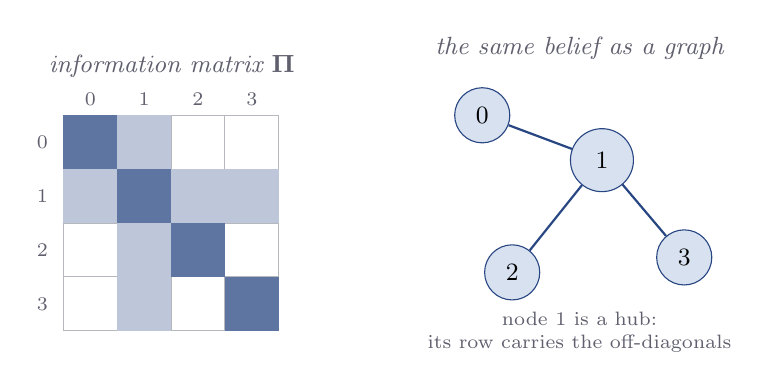
\begin{tikzpicture}[scale=0.95]
\def\g{0.72}
\begin{scope}
  \node[font=\small\itshape,grey] at (1.45,0.65) {information matrix $\Prec$};
  \foreach \i in {0,...,3}\foreach \j in {0,...,3}{
    \draw[grey!45] (\j*\g,-\i*\g) rectangle ++(\g,-\g);
  }
  \foreach \i in {0,...,3}{\fill[infomat!75] (\i*\g,-\i*\g) rectangle ++(\g,-\g);}
  % couplings among 0-1, 1-2, 1-3  (a hub at index 1)
  \foreach \i/\j in {0/1,1/0,1/2,2/1,1/3,3/1}{
    \fill[infomat!30] (\j*\g,-\i*\g) rectangle ++(\g,-\g);
  }
  \foreach \i in {0,...,3}{
    \node[font=\scriptsize,grey] at (-0.28,-\i*\g-0.36) {\i};
    \node[font=\scriptsize,grey] at (\i*\g+0.36,0.22) {\i};
  }
\end{scope}
% ---- right: the network
\begin{scope}[xshift=5.6cm,yshift=-1.0cm]
  \node[font=\small\itshape,grey] at (1.3,1.9) {the same belief as a graph};
  \node[circle,draw=infomat,fill=soft,minimum size=7mm,font=\small] (n0) at (0,1) {0};
  \node[circle,draw=infomat,fill=soft,minimum size=8mm,font=\small] (n1) at (1.6,0.4) {1};
  \node[circle,draw=infomat,fill=soft,minimum size=7mm,font=\small] (n2) at (0.4,-1.1) {2};
  \node[circle,draw=infomat,fill=soft,minimum size=7mm,font=\small] (n3) at (2.7,-0.9) {3};
  \draw[infomat,thick] (n0)--(n1);
  \draw[infomat,thick] (n1)--(n2);
  \draw[infomat,thick] (n1)--(n3);
  \node[font=\scriptsize,grey,align=center] at (1.3,-1.9)
     {node $1$ is a hub:\\ its row carries the off-diagonals};
\end{scope}
\end{tikzpicture}
\caption{The precision (information) matrix $\Prec$ \emph{is} the belief
network. Dark diagonal $=$ self-precision; light off-diagonal $=$
inferential coupling (an edge). A zero off-diagonal is a missing edge
(conditional independence). Node $1$ here is a hub --- a core node ---
because its row is full.}
\label{fig:matnet}
\end{figure}

Why this form and not mean--covariance? Because in this form
\emph{evidence is additive and combination is addition}. If two
independent sources of information about $\fvec$ have parameters
$(\Prec_1,\hvec_1)$ and $(\Prec_2,\hvec_2)$, the combined belief is
\begin{equation}
\Prec=\Prec_1+\Prec_2,\qquad \hvec=\hvec_1+\hvec_2.
\label{eq:add}
\end{equation}
Multiplying probability densities became \emph{adding} matrices. Hold onto
that --- it is the answer to ``when do I add something to the model.'' You
add to the model by adding to $\Prec$.

\begin{slogan}
A belief is an information matrix. To learn is to add to it. To
restructure is to border it or to Schur-complement it. To price the
restructuring is to evaluate a moment generating function.
\end{slogan}

% =====================================================================
\section{Three operations, not one: learn, expand, reduce}
% =====================================================================

The thing that tangles people --- you said this exactly --- is not knowing
\emph{when} you add to a model and when you remove. There are really three
distinct operations, and confusing them is the whole difficulty. Let me
separate them cleanly. Partition the parameters into a block we keep,
$\fvec_a$, and a block we are deciding about, $\fvec_b$, so that
\begin{equation}
\Prec=\begin{pmatrix}\Prec_{aa}&\Prec_{ab}\\[2pt]\Prec_{ba}&\Prec_{bb}\end{pmatrix},
\qquad
\hvec=\begin{pmatrix}\hvec_a\\ \hvec_b\end{pmatrix}.
\label{eq:block}
\end{equation}

\paragraph{(1) Learn --- add data.} Each observation deposits a little
information matrix $J_\tau$ (its Fisher information) and a potential
$\bm j_\tau$. By Eq.~\eqref{eq:add} the posterior after $t$ observations
is just a running sum,
\begin{equation}
\Prec(t)=\Prec_0+\sum_{\tau\le t}J_\tau,\qquad
\hvec(t)=\hvec_0+\sum_{\tau\le t}\bm j_\tau.
\label{eq:accum}
\end{equation}
Learning does not change the \emph{size} of the matrix, only its entries.
This is the dynamics; we return to it in \S\ref{sec:dynamics}.

\paragraph{(2) Expand --- add a parameter (your ``new'' node).} Now we add
a genuinely new degree of freedom $\fvec_b$ --- a new theoretical
commitment, a new node connected to the existing network. The matrix
\emph{grows}: we \emph{border} it with a new row and column whose entries
are the couplings $\Prec_{ab}$ of the newcomer to the incumbents
(Figure~\ref{fig:border}). The newcomer's conditionals $p(\,\text{node }k
\mid \text{new}\,)$ in your sketch are exactly these off-diagonal blocks.

\paragraph{(3) Reduce --- remove a parameter.} Here is the subtlety that
trips everyone: there are \emph{two} ways to remove $\fvec_b$, and they are
not the same.
\begin{itemize}
\item \textbf{Marginalize} (integrate it out). You keep believing the
newcomer might matter, but you no longer track it explicitly; you push its
information into correlations among the survivors. This is the
\emph{Schur complement} (\S\ref{sec:schur}).
\item \textbf{Prune} (assert it is absent). You sharpen its prior to a
spike --- declare the coupling zero --- and ask the data whether that
assertion costs you evidence. This is \emph{Bayesian model reduction}
proper (\S\ref{sec:bmr}), and the cost is the moment generating function
(\S\ref{sec:mgf}).
\end{itemize}
Marginalizing redistributes; pruning amputates and reads the bill. Most of
the confusion about BMR is really confusion between these two ``removes.''

\begin{figure}[ht]
\centering
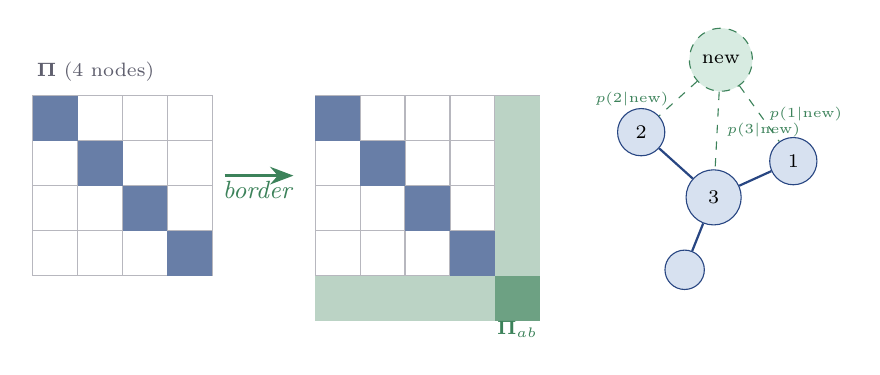
\begin{tikzpicture}[scale=0.92]
\def\g{0.62}
% 4x4 matrix
\begin{scope}
  \foreach \i in {0,...,3}\foreach \j in {0,...,3}{\draw[grey!45] (\j*\g,-\i*\g) rectangle ++(\g,-\g);}
  \foreach \i in {0,...,3}{\fill[infomat!70] (\i*\g,-\i*\g) rectangle ++(\g,-\g);}
  \node[font=\scriptsize,grey] at (1.4*\g,0.55*\g) {$\Prec$ (4 nodes)};
\end{scope}
% arrow
\node[addcol,font=\small\itshape] at (3.1,-1.3) {border};
\draw[->,addcol,very thick,>=Stealth] (2.65,-1.1) -- (3.6,-1.1);
% 5x5 matrix with last row/col highlighted
\begin{scope}[xshift=3.9cm]
  \foreach \i in {0,...,4}\foreach \j in {0,...,4}{\draw[grey!45] (\j*\g,-\i*\g) rectangle ++(\g,-\g);}
  \foreach \i in {0,...,3}{\fill[infomat!70] (\i*\g,-\i*\g) rectangle ++(\g,-\g);}
  \fill[addcol!75] (4*\g,-4*\g) rectangle ++(\g,-\g); % new diagonal
  \foreach \i in {0,...,3}{\fill[addcol!35] (4*\g,-\i*\g) rectangle ++(\g,-\g);} % new col
  \foreach \j in {0,...,3}{\fill[addcol!35] (\j*\g,-4*\g) rectangle ++(\g,-\g);} % new row
  \node[font=\scriptsize,addcol] at (4.5*\g,-5.2*\g) {$\Prec_{ab}$};
\end{scope}
% network on the right (mirrors the user's sketch)
\begin{scope}[xshift=8.4cm,yshift=-1.4cm]
  \node[circle,draw=infomat,fill=soft,minimum size=6mm,font=\scriptsize] (m2) at (0,0.9) {2};
  \node[circle,draw=infomat,fill=soft,minimum size=7mm,font=\scriptsize] (m3) at (1.0,0) {3};
  \node[circle,draw=infomat,fill=soft,minimum size=6mm,font=\scriptsize] (m1) at (2.1,0.5) {1};
  \node[circle,draw=infomat,fill=soft,minimum size=5mm] (mx) at (0.6,-1.0) {};
  \draw[infomat,thick] (m2)--(m3); \draw[infomat,thick] (m3)--(m1); \draw[infomat,thick] (m3)--(mx);
  \node[circle,draw=addcol,dashed,fill=softg,minimum size=8mm,font=\scriptsize] (nw) at (1.1,1.9) {new};
  \draw[addcol,dashed] (nw)--(m2) node[midway,left,font=\tiny]{$p(2|\text{new})$};
  \draw[addcol,dashed] (nw)--(m3) node[midway,right,font=\tiny]{$p(3|\text{new})$};
  \draw[addcol,dashed] (nw)--(m1) node[midway,right,font=\tiny]{$p(1|\text{new})$};
\end{scope}
\end{tikzpicture}
\caption{\textbf{Expansion is bordering.} Adding a new commitment grows
$\Prec$ by one row and column (green). The new diagonal is how strongly
the newcomer is believed on its own; the new off-diagonal block
$\Prec_{ab}$ holds its couplings to the incumbents --- exactly the
conditionals $p(k\mid\text{new})$ in the sketch. The dimension increases;
no incumbent entry is touched.}
\label{fig:border}
\end{figure}

% =====================================================================
\section{Removing by marginalizing: the Schur complement is the carry-over}
\label{sec:schur}
% =====================================================================

Suppose we decide to stop tracking $\fvec_b$ explicitly and integrate it
out. For a Gaussian this is exact, and in information form the answer is
the \emph{Schur complement}: the surviving block keeps precision
\begin{equation}
\Prec_{a}^{\text{marg}}
=\underbrace{\Prec_{aa}}_{\text{direct}}
-\underbrace{\Prec_{ab}\,\Prec_{bb}^{-1}\,\Prec_{ba}}_{\text{carry-over fill-in}},
\qquad
\hvec_a^{\text{marg}}=\hvec_a-\Prec_{ab}\Prec_{bb}^{-1}\hvec_b.
\label{eq:schur}
\end{equation}
Look at what the subtracted term does. Before, nodes that were coupled
only \emph{through} $\fvec_b$ had no direct edge. After we remove
$\fvec_b$, the term $\Prec_{ab}\Prec_{bb}^{-1}\Prec_{ba}$ writes new
off-diagonal entries among exactly those nodes (Figure~\ref{fig:schur}).
The removed node leaves its ghost behind as fresh couplings among its
former neighbours. \emph{This is the carry-over property, in one line of
linear algebra.} You cannot delete a hub cleanly; its influence
re-precipitates as correlations among everything it touched, and the more
it touched --- the larger $\Prec_{ab}$ --- the denser the ghost.

\begin{figure}[ht]
\centering
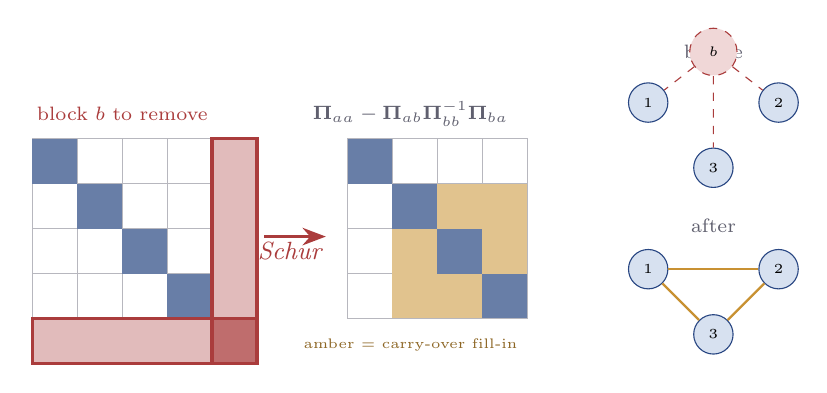
\begin{tikzpicture}[scale=0.92]
\def\g{0.62}
% 5x5 with b-block boxed
\begin{scope}
  \foreach \i in {0,...,4}\foreach \j in {0,...,4}{\draw[grey!45] (\j*\g,-\i*\g) rectangle ++(\g,-\g);}
  \foreach \i in {0,...,3}{\fill[infomat!70] (\i*\g,-\i*\g) rectangle ++(\g,-\g);}
  \fill[remcol!75] (4*\g,-4*\g) rectangle ++(\g,-\g);
  \foreach \i in {0,...,3}{\fill[remcol!35] (4*\g,-\i*\g) rectangle ++(\g,-\g);}
  \foreach \j in {0,...,3}{\fill[remcol!35] (\j*\g,-4*\g) rectangle ++(\g,-\g);}
  \draw[remcol,very thick] (4*\g,0) rectangle (5*\g,-5*\g);
  \draw[remcol,very thick] (0,-4*\g) rectangle (5*\g,-5*\g);
  \node[font=\scriptsize,remcol] at (2*\g,0.55*\g) {block $b$ to remove};
\end{scope}
\node[remcol,font=\small\itshape] at (3.55,-1.55) {Schur};
\draw[->,remcol,very thick,>=Stealth] (3.2,-1.35) -- (4.05,-1.35);
% 4x4 result with fill-in highlighted
\begin{scope}[xshift=4.35cm]
  \foreach \i in {0,...,3}\foreach \j in {0,...,3}{\draw[grey!45] (\j*\g,-\i*\g) rectangle ++(\g,-\g);}
  \foreach \i in {0,...,3}{\fill[infomat!70] (\i*\g,-\i*\g) rectangle ++(\g,-\g);}
  % fill-in among former neighbours (say nodes 1,2,3)
  \foreach \i/\j in {1/2,2/1,1/3,3/1,2/3,3/2}{\fill[amber!55] (\j*\g,-\i*\g) rectangle ++(\g,-\g);}
  \node[font=\scriptsize,grey] at (1.4*\g,0.55*\g) {$\Prec_{aa}-\Prec_{ab}\Prec_{bb}^{-1}\Prec_{ba}$};
  \node[font=\tiny,amber!70!black] at (1.4*\g,-4.6*\g) {amber $=$ carry-over fill-in};
\end{scope}
% networks
\begin{scope}[xshift=8.5cm,yshift=-0.3cm]
  \node[font=\scriptsize,grey] at (0.9,1.5) {before};
  \node[circle,draw=infomat,fill=soft,minimum size=5mm,font=\tiny] (a1) at (0,0.8) {1};
  \node[circle,draw=infomat,fill=soft,minimum size=5mm,font=\tiny] (a2) at (1.8,0.8) {2};
  \node[circle,draw=infomat,fill=soft,minimum size=5mm,font=\tiny] (a3) at (0.9,-0.1) {3};
  \node[circle,draw=remcol,dashed,fill=softr,minimum size=6mm,font=\tiny] (ab) at (0.9,1.5) {$b$};
  \draw[remcol,dashed](ab)--(a1);\draw[remcol,dashed](ab)--(a2);\draw[remcol,dashed](ab)--(a3);
\end{scope}
\begin{scope}[xshift=8.5cm,yshift=-2.6cm]
  \node[font=\scriptsize,grey] at (0.9,1.4) {after};
  \node[circle,draw=infomat,fill=soft,minimum size=5mm,font=\tiny] (c1) at (0,0.8) {1};
  \node[circle,draw=infomat,fill=soft,minimum size=5mm,font=\tiny] (c2) at (1.8,0.8) {2};
  \node[circle,draw=infomat,fill=soft,minimum size=5mm,font=\tiny] (c3) at (0.9,-0.1) {3};
  \draw[amber,thick](c1)--(c2);\draw[amber,thick](c1)--(c3);\draw[amber,thick](c2)--(c3);
\end{scope}
\end{tikzpicture}
\caption{\textbf{Reduction by marginalizing is the Schur complement.}
Integrating out block $b$ subtracts $\Prec_{ab}\Prec_{bb}^{-1}\Prec_{ba}$
from the survivors, which \emph{writes new edges} (amber) among $b$'s
former neighbours. The deleted node's influence does not vanish; it
re-precipitates as carry-over coupling. A hub leaves a dense ghost.}
\label{fig:schur}
\end{figure}

Two facts are worth saying out loud because they are the source of half
the practical pain.

\emph{First, a duality.} In \emph{covariance} form marginalizing is trivial
(delete rows) and conditioning is hard; in \emph{information} form it is
exactly reversed --- conditioning is trivial (delete rows of $\Prec$) and
marginalizing costs you the Schur complement. The two representations are
the same object rotated; whichever you pick, one of the two removals is
cheap and the other is the inverse you were hoping to avoid.

\emph{Second}, the Schur complement contains a matrix inverse,
$\Prec_{bb}^{-1}$. If $b$ is a single scalar this is a division; if $b$ is
a whole sub-network it is a genuine inversion. That is the first place the
``inverse Bayes is hard'' problem bites, and \S\ref{sec:compute} is about
why it usually does not bite as hard as it looks.

% =====================================================================
\section{Removing by pruning: Bayesian model reduction}
\label{sec:bmr}
% =====================================================================

Marginalizing answers ``what do I believe about the survivors if I stop
tracking $b$.'' It does \emph{not} answer ``should I have $b$ at all.''
For that we need the model \emph{evidence}, and the beautiful fact ---
the whole of BMR --- is that we can get the evidence of any
\emph{pruned} model from the full posterior we already computed, with no
re-fitting.

A pruned model has the \emph{same likelihood} but a different (sharper)
prior $\tilde p(\fvec)$ --- typically one that pins a coupling to zero.
Start from the two Bayes rules, solve the full one for the shared
likelihood, substitute into the reduced one, and integrate. In two lines
(this is Friston \& Penny's post-hoc identity, the matrix generalization
of the Savage--Dickey density ratio):
\begin{equation}
\boxed{\;\frac{\tilde \Z}{\Z}
=\E_{p(\fvec\mid y)}\!\left[\frac{\tilde p(\fvec)}{p(\fvec)}\right]\;}
\qquad\text{and}\qquad
\tilde p(\fvec\mid y)\;\propto\;p(\fvec\mid y)\,\frac{\tilde p(\fvec)}{p(\fvec)}.
\label{eq:bmr}
\end{equation}
\emph{The Bayes factor for any structural edit is the posterior
expectation of the prior ratio.} Everything on the right is already in
hand. No likelihood is re-evaluated; the posterior has already drunk the
data, and a prior change merely re-weights what it drank.

The sign of $\log(\tilde\Z/\Z)$ is the verdict. Sharpen the prior on a
coupling toward a spike at zero: if the data are content with the coupling
absent, the ratio exceeds one ($\log>0$) and you prune; if the data hold
the coupling away from zero, the ratio falls below one and you keep it.
This is automatic Occam: the complexity term of the free energy,
$\KL{p(\fvec\mid y)}{p(\fvec)}$, is exactly the price a parameter pays for
the prior volume it occupies, and pruning refunds that price whenever the
data did not need the volume.

% =====================================================================
\section{The ledger is a moment generating function}
\label{sec:mgf}
% =====================================================================

Now to the question you really asked: in density language, \emph{what is
the act of adding or removing}? It is \emph{exponential tilting}, and the
bill is the \emph{moment generating function}. Here is the cleanest case.

Multiply a belief $p(\fvec)$ by an exponential factor $e^{\bm t^{\top}\fvec}$
--- this is what ``adding a linear piece of evidence'' or ``adding a
coupling to a neighbour'' does to the density. The new normalizer is, by
definition,
\begin{equation}
\Z(\bm t)=\int p(\fvec)\,e^{\bm t^{\top}\fvec}\,d\fvec
=\E_{p}\!\big[e^{\bm t^{\top}\fvec}\big]
= M_p(\bm t),
\label{eq:mgf}
\end{equation}
the \emph{moment generating function} of $p$ evaluated at $\bm t$. To
\emph{add} the factor is to multiply the evidence by $M_p(\bm t)$; to
\emph{remove} it is to divide by $M_p(\bm t)$ --- tilt, and untilt. The
logarithm $K_p(\bm t)=\log M_p(\bm t)$ is the cumulant generating
function, and for a Gaussian it is the tidy quadratic
\begin{equation}
K_p(\bm t)=\bm\mu^{\top}\bm t+\tfrac12\,\bm t^{\top}\Cov\,\bm t,
\label{eq:cgf}
\end{equation}
whose first derivative is the mean and whose second is the covariance ---
the moments, generated. Compare Eq.~\eqref{eq:bmr}: the BMR Bayes factor is
$\E_{p(\fvec\mid y)}[\tilde p/p]$, and when the prior ratio is an
exponential-family tilt $\tilde p/p\propto e^{\bm t^{\top}\fvec}$ (a
mean-shift reduction), this expectation \emph{is} the posterior's MGF,
\begin{equation}
\frac{\tilde\Z}{\Z}=M_{p(\cdot\mid y)}(\bm t).
\label{eq:bmrmgf}
\end{equation}

\begin{slogan}
To add a belief is to tilt the distribution by an exponential; to remove
it is to tilt back. The evidence you gain or pay is the moment generating
function of what you already believe, read at the tilt. The
moment generating function is the ledger of structural change.
\end{slogan}

A pure precision change (pin a coupling, not just shift a mean) is the
generalized version: the prior ratio carries a quadratic
$e^{-\frac12\fvec^{\top}\Delta\Prec\,\fvec}$, and
$\E_{p(\cdot\mid y)}[\,\cdot\,]$ becomes the Gaussian integral of a
posterior against a quadratic tilt --- still an MGF-type object, now of
the squared parameter. The determinant and Mahalanobis terms in the
closed-form $\Delta F$ are precisely the $\log$ of that integral. So:
mean-shift edits are read off the MGF; precision edits are read off its
Gaussian generalization; both are the partition function
Eq.~\eqref{eq:mgf} doing its job.

% =====================================================================
\section{Why the inverse is hard, and the trick that saves you}
\label{sec:compute}
% =====================================================================

Bayes asks for a normalizer, $\Z=\int p(y\mid\fvec)p(\fvec)\,d\fvec$, and
for a Gaussian that means $\Z\propto|\Prec|^{-1/2}\exp(\tfrac12
\hvec^{\top}\Prec^{-1}\hvec)$ --- you need $\Prec^{-1}$, a $d\times d$
inverse, cost $O(d^3)$. Worse, naively scoring every candidate sub-model
means re-inverting a different matrix each time: $2^K$ structural edits,
each an $O(d^3)$ inversion. That is the wall people mean when they say
inverse Bayesian modelling is hard.

The escape is that structural edits are \emph{low-rank}. Pruning or adding
one edge changes $\Prec$ by a rank-one (or low-rank) bump
$\Prec\mapsto\Prec+\bm u\bm v^{\top}$, and the
Sherman--Morrison--Woodbury identity turns a low-rank change of a matrix
into a low-rank change of its \emph{already-computed} inverse,
\begin{equation}
(\Prec+\bm U\bm C\bm V)^{-1}
=\Prec^{-1}-\Prec^{-1}\bm U\big(\bm C^{-1}+\bm V\Prec^{-1}\bm U\big)^{-1}\bm V\Prec^{-1}.
\label{eq:woodbury}
\end{equation}
You pay the $O(d^3)$ inversion \emph{once}, for the full model; thereafter
each candidate edit is an $O(d^2)$ update, or cheaper for a single edge.
Schur complement (Eq.~\ref{eq:schur}) and Woodbury (Eq.~\ref{eq:woodbury})
are two faces of the same block-elimination identity --- the first removes
a block, the second patches the inverse when a block changes. \emph{BMR is
exactly the discipline of inverting once and updating forever.} That is
why it makes searching over paradigm topologies feasible at all: model
search collapses from ``solve $2^K$ inverse problems'' to ``solve one,
then evaluate $2^K$ algebraic expressions.''

% =====================================================================
\section{The dynamics: three theories chasing a moving world}
\label{sec:dynamics}
% =====================================================================

Now set it in motion. You have three candidate theories $A,B,C$. Each is a
generative model; each carries its own running information
$(\Prec^M(t),\hvec^M(t))$ accumulating by Eq.~\eqref{eq:accum}; each has a
running log-evidence $\log\Z^M(t)$. Two facts give the whole dynamical
picture.

\emph{Drift.} The expected one-step gain in a model's log-evidence, under
data from the true process $P$, is
\begin{equation}
\E_{P}\!\big[\log p_M(o)\big]=-H(P)-\KL{P}{p_M},
\label{eq:drift}
\end{equation}
so the \emph{rate} at which $\log\Z^M$ climbs is set, up to a common
constant, by $-\KL{P}{p_M}$: the model closest to the truth has the
steepest drift and pulls ahead. The running log-evidence of each theory is
a random walk with drift, and the drifts are ordered by Kullback--Leibler
distance from the world.

\emph{Switching.} If the world changes --- a regime shift, a new
phenomenon --- the KL distances re-order, the drifts re-order, and the
leading theory changes: a model-selection \emph{phase transition}
(Figure~\ref{fig:dynamics}). This is what you wanted to be able to
\emph{see}: you watch the three tallies $\log\Z^A,\log\Z^B,\log\Z^C$, and
the structure you should be running is the upper envelope --- whichever
curve is on top right now. The crossings are where paradigm change
happens.

\begin{figure}[ht]
\centering
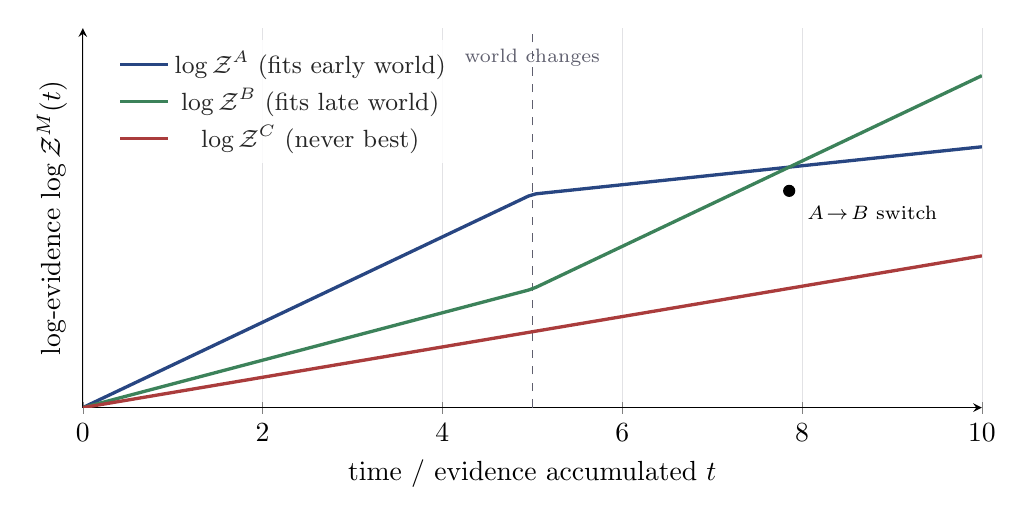
\begin{tikzpicture}
\begin{axis}[
  width=13cm,height=6.4cm,
  xlabel={time / evidence accumulated $t$},
  ylabel={log-evidence $\log\Z^M(t)$},
  xmin=0,xmax=10,ymin=0,ymax=8,
  xtick={0,2,4,6,8,10}, ytick=\empty,
  axis lines=left, grid=major, grid style={grey!18,very thin},
  legend pos=north west, legend style={font=\small,draw=none,fill=white,fill opacity=0.85},
  every axis plot/.append style={very thick},
]
% regime change marker
\draw[grey,dashed] (axis cs:5,0)--(axis cs:5,8);
\node[grey,font=\scriptsize,anchor=south] at (axis cs:5,7.0) {world changes};
% A: leads early (slope .9), flattens after (slope .2)
\addplot[infomat,domain=0:10,samples=120]{0.9*x-0.7*max(0,x-5)};
\addlegendentry{$\log\Z^A$ (fits early world)}
% B: slow early (.5), accelerates after (.9)
\addplot[addcol,domain=0:10,samples=120]{0.5*x+0.4*max(0,x-5)};
\addlegendentry{$\log\Z^B$ (fits late world)}
% C: mediocre throughout
\addplot[remcol,domain=0:10,samples=120]{0.32*x};
\addlegendentry{$\log\Z^C$ (never best)}
% switch point ~7.86
\fill[black] (axis cs:7.857,4.571) circle (2.2pt);
\node[font=\scriptsize,anchor=west] at (axis cs:7.95,4.1) {$A\!\to\!B$ switch};
\end{axis}
\end{tikzpicture}
\caption{\textbf{The dynamics you wanted to see.} Each theory's
log-evidence drifts at a rate set by its KL distance from the world
(Eq.~\ref{eq:drift}). Before the regime change $A$ is closest and leads;
after it, $B$'s drift is steeper and it overtakes $A$ at the crossing
(dot). The structure to run is the upper envelope; the crossing is a
paradigm shift. $C$ is dominated throughout and would be pruned.}
\label{fig:dynamics}
\end{figure}

The static moves of \S\S2--6 are how the agent \emph{responds} to this
flow. When the data start demanding a degree of freedom no current theory
has, the bordered (expanded) model's Bayes factor turns positive and the
agent \emph{adds} the node --- your ``new'' node arriving. When a coupling
goes silent, its pruning Bayes factor turns positive and the agent
\emph{removes} it. Expansion and reduction are the two controls by which a
believer keeps its information matrix aligned with a moving world; the
MGF (\S\ref{sec:mgf}) prices every move; Woodbury (\S\ref{sec:compute})
makes the pricing cheap enough to do continually.

% =====================================================================
\section{Rotating the object: expansion and reduction are adjoint}
% =====================================================================

Stand back and look at the one object from the two sides
(Figure~\ref{fig:rotate}). Bordering takes a $d\times d$ information matrix
to a $(d{+}1)\times(d{+}1)$ one by appending the couplings of a newcomer.
Schur-complementing takes it back, depositing the newcomer's influence as
carry-over among the survivors. They are inverse operations on the same
object: \emph{expansion is bordering; reduction is the Schur complement;
and they undo each other up to the ghost the removed node leaves behind.}
Bordering then immediately Schur-complementing the same block returns
$\Prec_{aa}$ exactly --- you get your money back if you remove what you
just added. Remove a node the data had \emph{used}, and the Schur term is
large: that is precisely an important node, and ``importance'' is now a
number --- the size of $\Prec_{ab}\Prec_{bb}^{-1}\Prec_{ba}$, the mass of
the off-diagonal block.

\begin{figure}[ht]
\centering
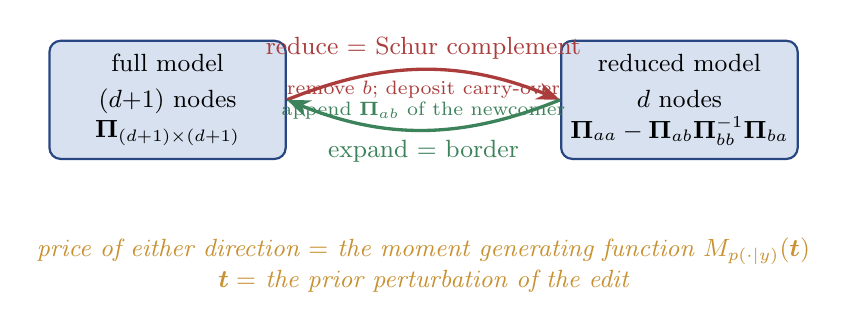
\begin{tikzpicture}[scale=1.0,>=Stealth]
\node[draw=infomat,thick,rounded corners,fill=soft,minimum width=3.0cm,minimum height=1.5cm,align=center,font=\small] (full)
  at (0,0) {full model\\[2pt]$(d{+}1)$ nodes\\ $\Prec_{(d+1)\times(d+1)}$};
\node[draw=infomat,thick,rounded corners,fill=soft,minimum width=3.0cm,minimum height=1.5cm,align=center,font=\small] (red)
  at (6.5,0) {reduced model\\[2pt]$d$ nodes\\ $\Prec_{aa}-\Prec_{ab}\Prec_{bb}^{-1}\Prec_{ba}$};
\draw[->,remcol,very thick] (full.east) to[bend left=22]
  node[above,font=\small,midway]{reduce $=$ Schur complement}
  node[below,font=\scriptsize,midway,remcol]{remove $b$; deposit carry-over} (red.west);
\draw[->,addcol,very thick] (red.west) to[bend left=22]
  node[below,font=\small,midway]{expand $=$ border}
  node[above,font=\scriptsize,midway,addcol]{append $\Prec_{ab}$ of the newcomer} (full.east);
\node[amber,font=\small\itshape,align=center] at (3.25,-2.1)
  {price of either direction $=$ the moment generating function $M_{p(\cdot\mid y)}(\bm t)$\\
   $\bm t=$ the prior perturbation of the edit};
\end{tikzpicture}
\caption{\textbf{One object, two rotations.} Expansion borders the
information matrix; reduction Schur-complements it. They are adjoint:
removing what you just added returns you exactly, and removing a
data-used (``important'') node leaves a large carry-over ghost. Either
direction is priced by the same moment generating function evaluated at
the edit's prior perturbation.}
\label{fig:rotate}
\end{figure}

% =====================================================================
\section{Reading your sketch in this language}
% =====================================================================

Now the ``Bayesian Model Expansion \& Reduction'' drawing maps cleanly,
stroke by stroke.

\begin{itemize}
\item \textbf{The core net (nodes $1,2,3$ and their solid edges)} is the
incumbent information matrix $\Prec_{aa}$ --- the current paradigm, the
block we keep.
\item \textbf{The dashed ``new'' node with its $p(1\mid\text{new}),
p(2\mid\text{new}),\dots$ edges} is a \emph{bordering}: a candidate column
$\Prec_{ab}$ of couplings appended to $\Prec_{aa}$
(Figure~\ref{fig:border}). The conditionals you wrote on those dashed
edges \emph{are} the entries of that column. Whether the node stays is
decided by Eq.~\eqref{eq:bmr}: compute the bordered model's Bayes factor
and read its sign.
\item \textbf{``new2''} on the right panel is a \emph{second, competing}
expansion --- a different candidate column. Expansion is not unique;
you propose several borderings and let the evidence
(Figure~\ref{fig:dynamics}) choose the upper envelope.
\item \textbf{The ``IMPORTANT NODE!''} that wires into many others is a hub
with a heavy off-diagonal block. Its importance is literal: marginalize it
and the carry-over fill-in $\Prec_{ab}\Prec_{bb}^{-1}\Prec_{ba}$ is large
(Figure~\ref{fig:schur}); you cannot remove it without massively
re-coupling its neighbours. High importance $=$ high carry-over $=$ a
large Schur correction $=$ a costly $\Delta F$ to prune.
\item \textbf{``Chris fields correct?''} --- the question of whether the
right primitive is a node that participates in conditionals across the net
--- is, in this language, the question of where to place the heavy
off-diagonal mass: is the proposed important node's column $\Prec_{ab}$
the one the evidence actually supports? That is answerable, and the
apparatus above is how: border it, score it by Eq.~\eqref{eq:bmr}, watch
its drift by Eq.~\eqref{eq:drift}.
\end{itemize}

So your picture and BMR are the same picture. Your drawing is the
\emph{expansion} half --- a new node reaching into the network through
conditionals. BMR is the \emph{reduction} half --- the Schur complement
that takes it back and the moment generating function that prices the
trip. Expansion borders; reduction Schur-complements; learning adds Fisher
information; the MGF keeps the books; Woodbury makes it cheap; and the
upper envelope of the competing log-evidences, drifting and crossing as
the world moves, is the paradigm you should be holding.

\appendix
% =====================================================================
\section{The carry-over matrix (Schur complement), slowly}
\label{app:schur}
% =====================================================================

The carry-over term $\Prec_{ab}\Prec_{bb}^{-1}\Prec_{ba}$ did a lot of work
above, so here is the same object built up from nothing, four ways, ending
in a worked example with actual numbers. The point to carry away: the
Schur complement is just \emph{what is left of one block after you
eliminate another}, and the elimination always leaves a residue --- that
residue is the carry-over.

\subsection{What it is: block elimination}

Take any block matrix and call the blocks $A,B,C,D$:
\begin{equation}
M=\begin{pmatrix}A&B\\ C&D\end{pmatrix}.
\end{equation}
You want to ``eliminate'' the $D$ corner the way you eliminate a variable
in ordinary Gaussian elimination --- use $D$ to clear the block above and
beside it. Doing that by block row/column operations factors $M$ exactly:
\begin{equation}
\begin{pmatrix}A&B\\ C&D\end{pmatrix}
=\begin{pmatrix}I&BD^{-1}\\ 0&I\end{pmatrix}
 \begin{pmatrix}\,M\schur D&0\\ 0&D\end{pmatrix}
 \begin{pmatrix}I&0\\ D^{-1}C&I\end{pmatrix},
\qquad
\boxed{\,M\schur D \;=\; A-BD^{-1}C\,}
\label{eq:schurdef}
\end{equation}
The middle factor is block-diagonal: $D$ sits in one corner, and in the
other corner sits $M\schur D=A-BD^{-1}C$, \emph{the Schur complement of
$D$ in $M$}. It is literally ``the $A$ block, corrected for everything that
ran through $D$.'' Two consequences fall out of Eq.~\eqref{eq:schurdef} by
taking determinants and inverting the triangular factors:
\begin{align}
\det M &= \det D \,\cdot\, \det(M\schur D), \label{eq:detsplit}\\
\big(M^{-1}\big)_{aa} &= (M\schur D)^{-1}. \label{eq:invblock}
\end{align}
Equation~\eqref{eq:detsplit} is why \emph{evidence factorises}: the
log-determinant of the information matrix splits into the part the removed
block carries and the part the survivors carry. Equation~\eqref{eq:invblock}
says the top-left block of the \emph{inverse} is the inverse of the Schur
complement --- the fact we use next.

\subsection{What it means: marginalize versus condition}

Put $M=\Prec$, the joint precision of $(\fvec_a,\fvec_b)$ as in
Eq.~\eqref{eq:block}. Now two different ``removals'' of $\fvec_b$ pick out
two different blocks, and this is the crux you said you wanted nailed down:

\begin{center}
\renewcommand{\arraystretch}{1.5}
\begin{tabular}{l|c|c}
 & \textbf{marginalize} $\fvec_b$ (integrate out) & \textbf{condition} on $\fvec_b$ (observe) \\\hline
\textbf{precision} $\Prec$ form & $\Prec_{aa}-\Prec_{ab}\Prec_{bb}^{-1}\Prec_{ba}$ \;(Schur) & $\Prec_{aa}$ \;(just the block) \\\hline
\textbf{covariance} $\Cov$ form & $\Cov_{aa}$ \;(just the block) & $\Cov_{aa}-\Cov_{ab}\Cov_{bb}^{-1}\Cov_{ba}$ \;(Schur)
\end{tabular}
\end{center}

Read the table across and a clean duality appears: \emph{the Schur
complement is the cost of the ``hard'' operation in each coordinate
system.} In precision coordinates, conditioning is free (you just keep the
$\Prec_{aa}$ block --- because the joint exponent already separates that
way) and \emph{marginalizing} costs the Schur complement. In covariance
coordinates it is exactly reversed. The reason marginalizing is the
expensive one in precision form is that integrating out a variable forces
you to account for everything that variable was holding together --- and
that accounting is $\Prec_{ab}\Prec_{bb}^{-1}\Prec_{ba}$.

\subsection{Where it comes from: completing the square}

This is the derivation worth remembering, because it shows the carry-over
being \emph{created}. The joint log-density has the quadratic
\begin{equation}
-\tfrac12
\begin{pmatrix}\fvec_a\\\fvec_b\end{pmatrix}^{\!\top}\!
\begin{pmatrix}\Prec_{aa}&\Prec_{ab}\\\Prec_{ba}&\Prec_{bb}\end{pmatrix}\!
\begin{pmatrix}\fvec_a\\\fvec_b\end{pmatrix}
=-\tfrac12\Big[\fvec_a^{\top}\Prec_{aa}\fvec_a
+2\fvec_a^{\top}\Prec_{ab}\fvec_b
+\fvec_b^{\top}\Prec_{bb}\fvec_b\Big].
\end{equation}
To marginalize $\fvec_b$ we integrate it out, and to integrate a Gaussian
we complete the square in $\fvec_b$. The two $\fvec_b$ terms combine as
\begin{equation}
\fvec_b^{\top}\Prec_{bb}\fvec_b+2\fvec_a^{\top}\Prec_{ab}\fvec_b
=\underbrace{\big(\fvec_b+\Prec_{bb}^{-1}\Prec_{ba}\fvec_a\big)^{\!\top}
\Prec_{bb}\big(\fvec_b+\Prec_{bb}^{-1}\Prec_{ba}\fvec_a\big)}_{\text{integrates away to a constant}}
\;-\;\fvec_a^{\top}\,\Prec_{ab}\Prec_{bb}^{-1}\Prec_{ba}\,\fvec_a.
\end{equation}
The shifted-square term, integrated over $\fvec_b$, gives just a
normalising constant. What \emph{stays behind}, glued to $\fvec_a$, is the
second piece. So the marginal of $\fvec_a$ has quadratic
\begin{equation}
-\tfrac12\,\fvec_a^{\top}\big(\Prec_{aa}-\Prec_{ab}\Prec_{bb}^{-1}\Prec_{ba}\big)\fvec_a,
\end{equation}
and there it is: \emph{the Schur complement is the residue that completing
the square cannot remove.} The carry-over $\Prec_{ab}\Prec_{bb}^{-1}\Prec_{ba}$
is precisely the imprint $\fvec_b$ leaves on $\fvec_a$ when you push it out
of the model --- not a modelling choice, a remainder term.

\subsection{A worked example you can see}

Take the smallest interesting case: a \emph{star}. Two outer nodes $1,2$
each couple to a central hub $b$, and crucially $1$ and $2$ have
\emph{no direct edge} between them ($\Prec_{12}=0$). In the ordering
$(1,2,b)$, with self-precisions $2$ and unit couplings to the hub,
\begin{equation}
\Prec=\begin{pmatrix}2&0&1\\ 0&2&1\\ 1&1&2\end{pmatrix},
\qquad
\Prec_{aa}=\begin{pmatrix}2&0\\0&2\end{pmatrix},\;
\Prec_{ab}=\begin{pmatrix}1\\1\end{pmatrix},\;
\Prec_{bb}=2,\;
\Prec_{ba}=\begin{pmatrix}1&1\end{pmatrix}.
\end{equation}
Marginalize the hub $b$. The carry-over matrix is a rank-one outer product
(because $b$ is one node):
\begin{equation}
\Prec_{ab}\Prec_{bb}^{-1}\Prec_{ba}
=\frac{1}{2}\begin{pmatrix}1\\1\end{pmatrix}\begin{pmatrix}1&1\end{pmatrix}
=\begin{pmatrix}0.5&0.5\\0.5&0.5\end{pmatrix},
\end{equation}
and the surviving precision is
\begin{equation}
\Prec_{aa}-\Prec_{ab}\Prec_{bb}^{-1}\Prec_{ba}
=\begin{pmatrix}2&0\\0&2\end{pmatrix}-\begin{pmatrix}0.5&0.5\\0.5&0.5\end{pmatrix}
=\begin{pmatrix}\,1.5&-0.5\,\\[1pt]\,-0.5&1.5\,\end{pmatrix}.
\end{equation}
Two things happened (Figure~\ref{fig:star}). \textbf{An edge was born}: the
off-diagonal went from $0$ to $-0.5$ --- nodes $1$ and $2$, which had no
direct coupling, are now coupled, purely because they both leaned on $b$.
And \textbf{each node lost precision}: the diagonal fell $2\to1.5$, because
the hub was helping pin them and now it is gone. The induced coupling is
$\Prec_{1b}\Prec_{bb}^{-1}\Prec_{b2}=c_1 c_2/d$ --- the product of the two
couplings to the hub, divided by the hub's own precision. A hub that many
nodes lean on hard (large $\Prec_{ab}$) leaves a large, dense induced
block: \emph{that} is what makes a node ``important,'' and why an
important node is expensive to remove.

\begin{figure}[ht]
\centering
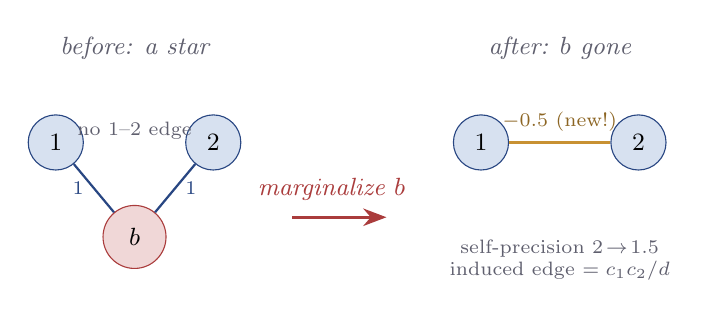
\begin{tikzpicture}[scale=1.0]
% before: star
\begin{scope}
  \node[font=\small\itshape,grey] at (1.0,2.2) {before: a star};
  \node[circle,draw=infomat,fill=soft,minimum size=7mm,font=\small] (o1) at (0,1) {1};
  \node[circle,draw=infomat,fill=soft,minimum size=7mm,font=\small] (o2) at (2,1) {2};
  \node[circle,draw=remcol,fill=softr,minimum size=8mm,font=\small] (hb) at (1,-0.2) {$b$};
  \draw[infomat,thick] (o1)--(hb) node[midway,left,font=\scriptsize]{$1$};
  \draw[infomat,thick] (o2)--(hb) node[midway,right,font=\scriptsize]{$1$};
  \node[font=\scriptsize,grey] at (1,1.15) {no $1$--$2$ edge};
\end{scope}
% arrow
\node[remcol,font=\small\itshape] at (3.5,0.4) {marginalize $b$};
\draw[->,remcol,very thick,>=Stealth] (3.0,0.05) -- (4.2,0.05);
% after: induced edge
\begin{scope}[xshift=5.4cm]
  \node[font=\small\itshape,grey] at (1.0,2.2) {after: $b$ gone};
  \node[circle,draw=infomat,fill=soft,minimum size=7mm,font=\small] (p1) at (0,1) {1};
  \node[circle,draw=infomat,fill=soft,minimum size=7mm,font=\small] (p2) at (2,1) {2};
  \draw[amber,very thick] (p1)--(p2) node[midway,above,font=\scriptsize,amber!70!black]{$-0.5$ (new!)};
  \node[font=\scriptsize,grey,align=center] at (1,-0.5)
    {self-precision $2\!\to\!1.5$\\ induced edge $=c_1c_2/d$};
\end{scope}
\end{tikzpicture}
\caption{\textbf{The carry-over, with numbers.} Marginalizing the hub $b$
of a star induces a direct edge ($-0.5$) between its two formerly
unconnected neighbours and drops their self-precision ($2\to1.5$). The
induced coupling is the product of the couplings to $b$ over $b$'s own
precision --- big for a heavily-leaned-on hub. This is the carry-over
matrix $\Prec_{ab}\Prec_{bb}^{-1}\Prec_{ba}$ doing its one job.}
\label{fig:star}
\end{figure}

\subsection{The name the numerical analysts use: fill-in}

That born edge has a name in sparse linear algebra: \emph{fill-in}. When
Gaussian elimination (or Cholesky) eliminates a variable, it connects all
of that variable's neighbours to each other --- new nonzeros appear where
the original matrix had zeros. The Schur complement \emph{is} one
elimination step, and the carry-over \emph{is} its fill-in. This buys two
things for the paradigm story:

\begin{itemize}
\item \textbf{Importance $=$ fill-in.} A node whose elimination produces a
lot of fill-in is one whose removal re-wires the whole network --- exactly
the heavy-Schur-correction ``important node'' of \S9. Belt nodes eliminate
cheaply (few neighbours, little fill-in); core hubs eliminate expensively
(many neighbours, dense fill-in).
\item \textbf{Elimination order is belt-first.} Numerical analysts choose
the elimination ordering that minimises fill-in (minimum-degree and nested
dissection orderings). For a core/belt network that ordering is precisely
\emph{belt-first, core-last} --- which is the same belt-first, core-last
sequence the structural reorganisation follows in the population dynamics.
The cheapest way to take a paradigm apart and the order in which a
community actually takes it apart are the same order, and for the same
reason: you do the low-fill-in moves first.
\end{itemize}

\noindent Finally, tie it back to the paper's carry-over cost. The
propagating revision cost $C(v)$ written there as ``local KL plus
precision-weighted downstream KLs, summed over the cascade'' is the
\emph{series-expansion} reading of the same object: iterating the Schur
elimination one neighbour at a time generates exactly that sum, and the
closed form of the whole cascade is the single matrix
$\Prec_{ab}\Prec_{bb}^{-1}\Prec_{ba}$. The cascade picture and the Schur
picture are the same carry-over, told step-by-step versus all-at-once.

% =====================================================================
\section{The tilt, and why the moment generating function is its price}
\label{app:tilt}
% =====================================================================

You said the tilt is the part you cannot see. Let us draw it. There is
really one move and one picture: \emph{multiply a density by an
exponential, and renormalize.} Everything else --- adding evidence,
removing a coupling, scoring a model --- is that move, and the MGF is the
bill it leaves.

\subsection{The move: multiply by an exponential, then renormalize}

Start with a belief $p(\fvec)$ and a ``tilt'' $e^{\bm t^{\top}\fvec}$. This
factor is a wager: it pays off exponentially more for large $\bm
t^{\top}\fvec$, so multiplying by it up-weights one side of your belief and
down-weights the other (Figure~\ref{fig:tilt}, left). The product
$p(\fvec)\,e^{\bm t^{\top}\fvec}$ is no longer a probability density --- it
does not integrate to one --- so you divide by whatever it \emph{does}
integrate to. That number is the MGF, and the renormalized object is the
\emph{tilted} density:
\begin{equation}
p_{\bm t}(\fvec)=\frac{p(\fvec)\,e^{\bm t^{\top}\fvec}}{M_p(\bm t)},
\qquad
M_p(\bm t)=\int p(\fvec)\,e^{\bm t^{\top}\fvec}\,d\fvec
=\E_p\!\big[e^{\bm t^{\top}\fvec}\big].
\label{eq:tiltdef}
\end{equation}
So the MGF is, quite literally, \emph{the area you sweep up when you tilt}
--- the total mass of the wagered density. To \emph{add} the wager to your
model is to pay that area; to \emph{remove} it is to tilt back by $-\bm t$
and divide it out.

\begin{figure}[ht]
\centering
\begin{minipage}{0.49\textwidth}\centering
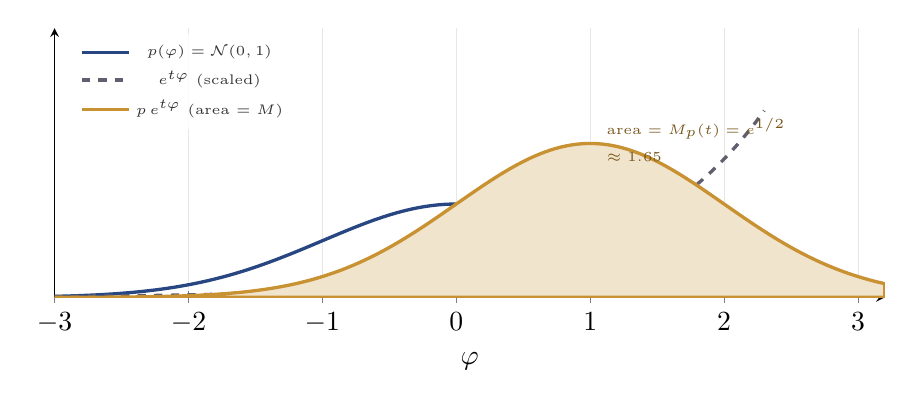
\begin{tikzpicture}
\begin{axis}[width=\textwidth,height=5.0cm,
  xlabel={$\varphi$},ylabel={},xmin=-3,xmax=3.2,ymin=0,ymax=1.15,
  ytick=\empty,axis lines=left,grid=major,grid style={grey!15,very thin},
  legend style={font=\tiny,draw=none,fill=white,fill opacity=0.8,at={(0.02,0.98)},anchor=north west},
  every axis plot/.append style={very thick}]
% original p = N(0,1)
\addplot[infomat,domain=-3:3.2,samples=120]{1/sqrt(2*pi)*exp(-x^2/2)};
\addlegendentry{$p(\varphi)=\mathcal N(0,1)$}
% tilt factor, scaled, restricted
\addplot[grey,dashed,domain=-3:2.3,samples=80]{0.08*exp(x)};
\addlegendentry{$e^{t\varphi}$ (scaled)}
% product, unnormalized: peaks at x=1
\addplot[amber,fill=amber!25,domain=-3:3.2,samples=160]{1/sqrt(2*pi)*exp(-x^2/2+x)}\closedcycle;
\addlegendentry{$p\,e^{t\varphi}$ (area $=M$)}
\node[font=\tiny,amber!60!black,anchor=west] at (axis cs:1.05,0.72) {area $=M_p(t)=e^{1/2}$};
\node[font=\tiny,amber!60!black,anchor=west] at (axis cs:1.05,0.60) {$\approx 1.65$};
\end{axis}
\end{tikzpicture}\\[1pt]
{\footnotesize (a) multiply: the swept area is the MGF}
\end{minipage}\hfill
\begin{minipage}{0.49\textwidth}\centering
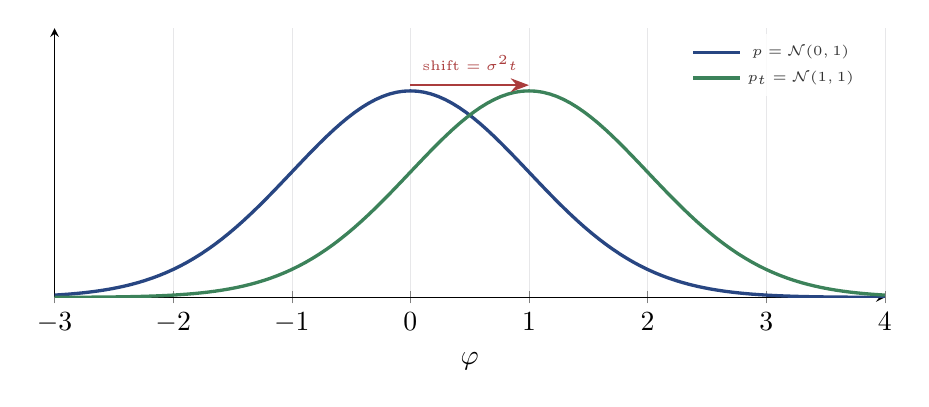
\begin{tikzpicture}
\begin{axis}[width=\textwidth,height=5.0cm,
  xlabel={$\varphi$},ylabel={},xmin=-3,xmax=4,ymin=0,ymax=0.52,
  ytick=\empty,axis lines=left,grid=major,grid style={grey!15,very thin},
  legend style={font=\tiny,draw=none,fill=white,fill opacity=0.8,at={(0.98,0.98)},anchor=north east},
  every axis plot/.append style={very thick}]
\addplot[infomat,domain=-3:4,samples=120]{1/sqrt(2*pi)*exp(-x^2/2)};
\addlegendentry{$p=\mathcal N(0,1)$}
\addplot[addcol,domain=-3:4,samples=120]{1/sqrt(2*pi)*exp(-(x-1)^2/2)};
\addlegendentry{$p_t=\mathcal N(1,1)$}
\draw[->,remcol,thick,>=Stealth] (axis cs:0,0.41)--(axis cs:1,0.41);
\node[font=\tiny,remcol,anchor=south] at (axis cs:0.5,0.42) {shift $=\sigma^2 t$};
\end{axis}
\end{tikzpicture}\\[1pt]
{\footnotesize (b) renormalize: a rigid shift of the bump}
\end{minipage}
\caption{\textbf{The tilt, drawn.} (a) Multiplying the belief
$p=\mathcal N(0,1)$ by $e^{t\varphi}$ (here $t=1$) up-weights the right and
makes the un-normalized product (amber); the \emph{area} under that
product is the moment generating function $M_p(t)=e^{1/2}\approx1.65$ ---
the evidence you pay for the wager. (b) Renormalizing gives back a genuine
density $p_t$, which for a Gaussian is just the original \emph{rigidly
shifted} by $\sigma^2 t$, same width. To remove the wager you tilt by
$-t$ and shift back.}
\label{fig:tilt}
\end{figure}

\subsection{For a Gaussian, the tilt is a rigid shift}

Complete the square in Eq.~\eqref{eq:tiltdef} with $p=\mathcal N(\bm\mu,\Cov)$
and you find the tilt does something very simple --- it slides the mean and
leaves the shape alone:
\begin{equation}
p_{\bm t}=\mathcal N\!\big(\bm\mu+\Cov\bm t,\ \Cov\big),
\qquad
M_p(\bm t)=\exp\!\Big(\bm\mu^{\top}\bm t+\tfrac12\bm t^{\top}\Cov\bm t\Big),
\qquad
K_p(\bm t)=\bm\mu^{\top}\bm t+\tfrac12\bm t^{\top}\Cov\bm t.
\label{eq:gausstilt}
\end{equation}
The mean moves by $\Cov\bm t$: \emph{the more uncertain you are, the more a
given wager moves you} (a broad belief is easily tilted; a sharp one
barely budges). That is the whole content of Figure~\ref{fig:tilt}(b), and
it is why high-variance --- low-precision --- beliefs are the ones the data,
or a neighbour, can shift.

\subsection{The CGF is the ledger; its derivatives are the moments}

Take logs: $K_p(\bm t)=\log M_p(\bm t)$, the cumulant generating function,
is the actual ledger. For one parameter it is the parabola
$K(t)=\mu t+\tfrac12\sigma^2 t^2$ (Figure~\ref{fig:cgf}), and three things
are worth reading off it:
\begin{equation}
K(0)=0,\qquad
K'(0)=\mu,\qquad
K''(0)=\sigma^2.
\end{equation}
At no tilt there is no cost. The \emph{slope at the origin is the mean};
the \emph{curvature is the variance}. This is what ``moment generating''
means made visible: differentiate the ledger and the moments fall out.
More: $K'(\bm t)=\E_{p_{\bm t}}[\fvec]$ is the mean of the \emph{tilted}
distribution, so as you crank the field $\bm t$ the slope of the ledger
traces where the tilted bump has moved to. And the height $K(\bm t)$ at a
chosen tilt is simply the log-evidence you pay for that edit. One curve
holds the price, the mean, and the variance at once.

\begin{figure}[ht]
\centering
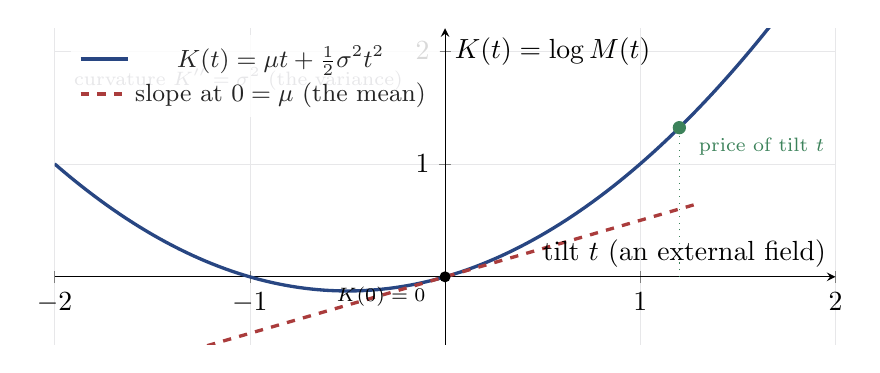
\begin{tikzpicture}
\begin{axis}[width=11.5cm,height=5.6cm,
  xlabel={tilt $t$ (an external field)},ylabel={$K(t)=\log M(t)$},
  xmin=-2,xmax=2,ymin=-0.6,ymax=2.2,
  axis lines=middle,grid=major,grid style={grey!15,very thin},
  every axis plot/.append style={very thick},
  xtick={-2,-1,1,2}, ytick={1,2},
  legend style={font=\small,draw=none,fill=white,fill opacity=0.85,at={(0.02,0.98)},anchor=north west}]
% CGF parabola mu=0.5 sigma2=1
\addplot[infomat,domain=-2:2,samples=120]{0.5*x+0.5*x^2};
\addlegendentry{$K(t)=\mu t+\tfrac12\sigma^2 t^2$}
% tangent at origin slope mu=0.5
\addplot[remcol,dashed,domain=-1.3:1.3,samples=2]{0.5*x};
\addlegendentry{slope at $0=\mu$ (the mean)}
% origin marker
\fill[black] (axis cs:0,0) circle (2pt);
\node[font=\scriptsize,anchor=north east] at (axis cs:-0.05,0.0) {$K(0)=0$};
% price marker at t=1.2 -> K=0.6+0.72=1.32
\fill[addcol] (axis cs:1.2,1.32) circle (2.4pt);
\draw[addcol,dotted] (axis cs:1.2,0)--(axis cs:1.2,1.32);
\node[font=\scriptsize,addcol,anchor=west] at (axis cs:1.25,1.15) {price of tilt $t$};
% curvature note
\node[font=\scriptsize,grey,anchor=west] at (axis cs:-1.95,1.75) {curvature $K''=\sigma^2$ (the variance)};
\end{axis}
\end{tikzpicture}
\caption{\textbf{The ledger.} The cumulant generating function $K(t)$ ---
for a Gaussian a parabola --- prices every tilt. It passes through the
origin (no tilt, no cost); its slope there is the mean; its curvature is
the variance; and its height at a chosen tilt $t$ is the log-evidence that
edit costs. Differentiating the ledger generates the moments --- the
literal meaning of ``moment generating.''}
\label{fig:cgf}
\end{figure}

\subsection{Three ways to read the same tilt}

The picture is robust because it is the same object physicists,
statisticians, and probabilists each met under a different name.
\begin{itemize}
\item \textbf{Change of measure (statistics).} The tilted density relative
to the original is $\dfrac{dp_{\bm t}}{dp}(\fvec)=\dfrac{e^{\bm
t^{\top}\fvec}}{M_p(\bm t)}$ --- a Radon--Nikodym derivative. Tilting is
re-weighting one measure into another; importance sampling is exactly this
re-weight. And this is why BMR is an MGF: the prior ratio $\tilde
p/p$ in Eq.~\eqref{eq:bmr} \emph{is} a tilt factor, so $\tilde\Z/\Z=\E_{p(\cdot\mid
y)}[\tilde p/p]$ is the posterior's MGF at that tilt --- model scoring
\emph{is} measuring the area you sweep when you re-weight your posterior by
the proposed prior change.
\item \textbf{Laplace transform (analysis).} $M_p(\bm t)=\int e^{\bm
t^{\top}\fvec}p(\fvec)\,d\fvec$ is the (two-sided) Laplace transform of the
density. Tilting-and-reading-the-MGF is taking a transform; the
inversion that recovers $p$ from $M$ is the hard direction --- the same
``inverse is hard'' theme of \S\ref{sec:compute}.
\item \textbf{External field / free energy (physics).} Read $\bm t$ as an
external field that couples linearly to $\fvec$. Then $M_p(\bm t)=Z(\bm t)$
is a partition function, $K_p(\bm t)=\log Z$ is (minus) a free energy, and
its derivatives are the response functions: $K'$ is the magnetization (the
mean), $K''$ is the susceptibility (the variance). \emph{Adding a belief is
turning on a field; the evidence you pay is the free-energy change; the
moments are how the system responds.} For a project built on free energy,
this is the tilt's home: the MGF ledger and the variational free energy are
the same bookkeeping, one in the space of beliefs, the other in the space
of fields.
\end{itemize}

\noindent So the slogan of \S\ref{sec:mgf} is now a picture you can hold.
To add a belief is to tilt the bump (Figure~\ref{fig:tilt}); the area you
sweep is the MGF; the ledger $K$ (Figure~\ref{fig:cgf}) charges you its
height and hands you the mean and variance as its slope and curvature; and
to remove the belief you tilt back and the area divides out. Expansion,
reduction, and learning are all the same hand on the same dial --- and the
dial is a field, the meter is a free energy.

\end{document}
